\documentclass[12pt,a4paper]{report}
\usepackage{geometry}
\geometry{top=14mm, bottom=15mm}
\usepackage[english]{babel}
\usepackage[utf8]{inputenc}
\usepackage{fancyhdr}
\usepackage{csquotes}
\usepackage{listings}
\usepackage{hyperref}
\usepackage{graphics, graphicx}
\usepackage{graphics, graphicx}
\usepackage{amsmath}
\pagestyle{fancy}

\fancyhf{}
%\rhead{}
%\lhead{}
\fancyfoot[LE,LO]{Data Analytics}
\fancyfoot[RE,RO]{Mini Project - 4}
\renewcommand{\footrulewidth}{1pt}
 \medskip
 \author{Abhijeet Singh Panwar (ID : 201351005)}
\title{Data Analytics\\ Mini Project - 4}

\date{\parbox{\linewidth}{\centering%
  \today\endgraf\bigskip
  Instructor : \endgraf\medskip
  Prof. Bhargab Chattopadhyay\endgraf\bigskip
  Indian Institute of Information Technology, Vadodara}}
\begin{document}
\maketitle
\newpage
\section{Question 1}
\textbf{Consider the dataset stored in the file bp.xlsx. This dataset contains one measurement of systolic blood pressure (in mmHg) made by each of two methods — a finger method and an arm method — from the same
200 patients.}
\\\\
\textbf{Part A}
\\\\
Perform an exploratory analysis of the data by examining the distributions of the measurements from the two methods using boxplots. Comment on what you see. Do the two distributions seem similar? Justify your answer.
\\\\
\textbf{Solution}
\\\\
\begin{figure}[h]
\begin{center}
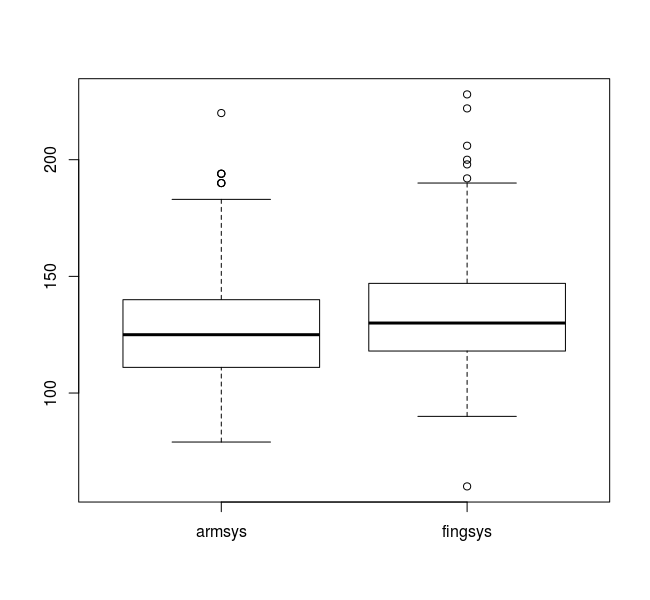
\includegraphics[scale=0.5]{plot.png}
\caption{Box-plot of Fingsys \& Armsys}
\end{center}
\end{figure}
From boxplot, we can observe that spread(or variance) of both the distribution, are nearly equal.
\\\\
\textbf{Part B}
\\\\
Use histograms and QQ plots to examine the shapes of the two distributions. Comment on what you see. Does the assumption of normality seem reasonable? Justify your answer.
\\\\
\textbf{Solution}
\\\\
\begin{figure}
$
\begin{array}{cc}
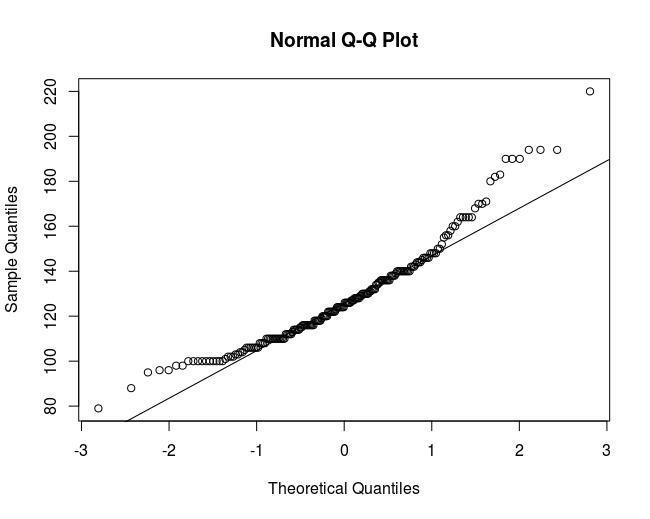
\includegraphics[width=2.5 in]{armsys.png} &
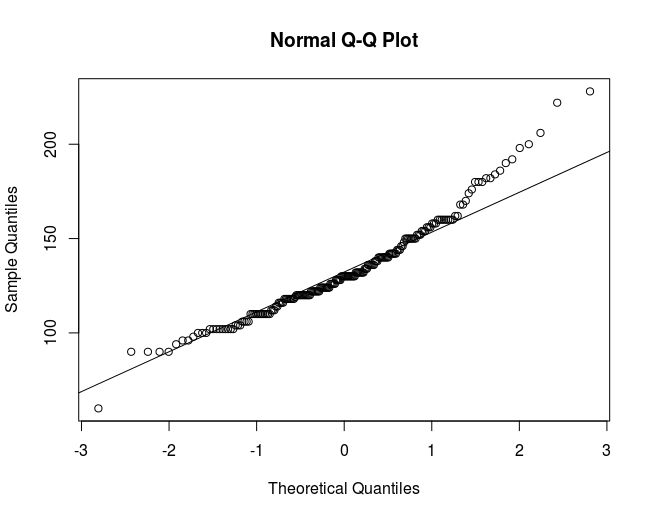
\includegraphics[width=2.5 in]{fingsys.png}
\end{array}$
\caption{Q-Q plot of both Armsys \& Fingsys}
$
\begin{array}{cc}
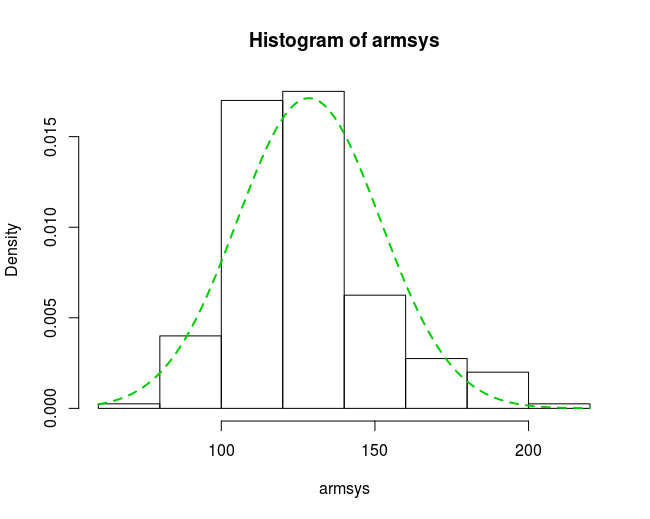
\includegraphics[width=2.5 in]{armsys_hist.png} &
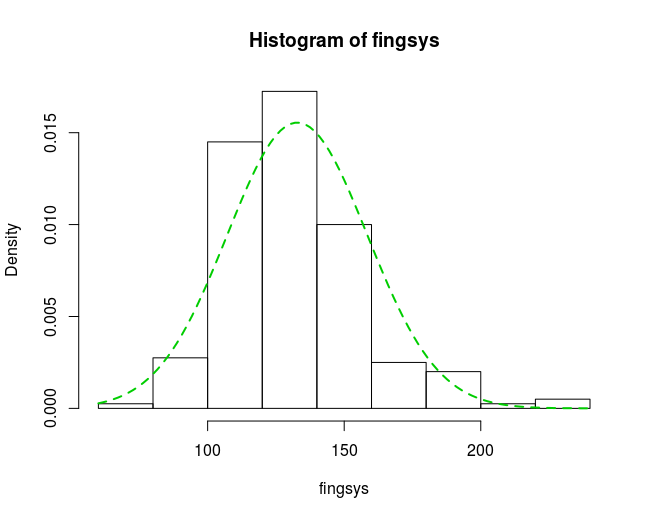
\includegraphics[width=2.5 in]{fingsys_hist.png}
\end{array}$
\caption{Q-Q plot of both Armsys \& Fingsys}
\end{figure}
\newpage
From seeing both, qqplot \& histogram for \textbf{Armsys} \& \textbf{Fingsys}, \textbf{it is evident that both the distributions are normal in nature}. Hence, in case of qqplot, more the points are towards y=x line, more the chances of given dataset to be normal in nature. Similarly, in case of histogram for both dataset, the normal curve nearly fits the histogram.
\\\\
\textbf{Part C}
\\\\
Construct an appropriate 95\% confidence interval for the difference in the means of the two methods. Interpret your results. Can we conclude that the two methods have identical means? Justify your answer. What assumptions, if any, did you make to construct the interval? Do the assumptions seem to hold?
\\\\
\textbf{Solution}
\\\\
\textbf{Assumption}
\begin{enumerate}
\item Variance of both distribution are equal.  \textit{Reffered to Part B}
\end{enumerate}

\textit{The confidence interval for difference of mean of two distribution is}:\\
\begin{center}
$\lbrack -72.19, 63.60 \rbrack$
\end{center}
\textbf{Part D}
\\\\
Perform an appropriate 5\% level test to see if there is any difference in the means of the two methods. Be sure to clearly set up the null and alternative hypotheses. State your conclusion. What assumptions, if any, did you make to construct the interval? Do they seem to hold?
\\\\
\textbf{Solution}
\\\\
Null Hypothesis($H_o$) : $(mean)_{Armsys} - (mean)_{Fingsys} = 0$\\\\
Alternative Hypothesis($H_a$) : $(mean)_{Armsys} - (mean)_{Fingsys}$  $\neq$ 0\\\\
For, $\alpha$ = 0.05
\\\\
We will use t-test for hypothesis testing, as in this case population variace is unknown \& assumed to be equal for both distribution.\\\\
Test statistic(t) = $(mean)_{Armsys} - (mean)_{Fingsys} \div S_p * \sqrt{1/n + 1/m}$\\\\
Here, $S_p$, is pooled sample variance.\\
n, is size of Armsys distribution.\\
m, is size of Fingsys distribution.\\
\\
If $\mid t \mid >$ PValue, we reject Null Hypothesis,\\\\
Through calculation,\\\\
t, comes out to be -0.00715 \& PValue comes out to be 1.965.\\\\
Therefore, null hypothesis is accepted, this shows that there is no difference in means of two methods.
\\\\
\textbf{Part E}
\\\\
Do the results from (c) and (d) seem consistent? Justify your answer.
\\\\
\textbf{Solution}
\\\\
%put solution here
\\\\
\section{Question 2}
\textbf{Suppose we are interested in testing the null hypothesis that the mean of a normal population is 10 against the alternative that it is greater than 10. A random sample of size 20 from this population gives 9.02 as the sample mean and 2.22 as the sample standard deviation.}
\\\\
\textbf{Part A}
\\\\
Set up the null and alternative hypotheses.
\\\\
\textbf{Solution}\\\\
The null hypothesis($H_o$) will be : $\mu$ = 10, where $\mu$ is population mean.\\
And, the alternative hypothesis($H_a$) will be $\mu$ $>$ 10.
\\\\
\textbf{Part B}
\\\\
Which test would you use? What is the test statistic? What is the null distribution of the test statistic?
\\\\
\textbf{Solution}
\\\\
T-tests will be implemented, as population variance($\sigma$) is unknown.\\\\
Therefore, the test-statistic(t) will be, ($\overline{X} - \mu _o) \div s/\sqrt{n}$.\\\\
Here, \textit{$\overline{X}$ is sample mean,\\ and n is sample size}.\\\\
Student's T-distribution will be the null distribution for out test statistic.
\\\\
\textbf{Part C}
\\\\
Compute the observed value of the test statistic.
\\\\
\textbf{Solution}
\\\\
Value of test statistic based on above formula will be, \textbf{-1.974186}
\\\\
\textbf{Part D}
\\\\
Compute the p-value of the test using the usual way.
\\\\
\textbf{Solution}
\\\\
P-values for T-tests ($F_\nu$ is the cdf of T-distribution with the suitable number $\nu$ of degrees of freedom).\\\\
Therefore, using the formula $\rightarrow$ 1 - $F_{a} (t_{obs})$.\\\\
P-value = 0.03153941
\\\\
\textbf{Part E}
\\\\
Estimate the p-value of the test using Monte Carlo simulation. How do your answers in (d) and (e) compare?
\\\\
\textbf{Solution}
\\\\
From Monte Carlo estimation, the p-value thus obtained is 0.0344. And, pvalue calculated from two different methods, comes out to be nearly equal.
\\\\
\textbf{Part F}
\\\\
State your conclusion at 5\% level of significance.
\\\\
\textbf{Solution}
\\\\
As, $\alpha$ $\rightarrow$ 0.05, is greater than $P\_ value$, i.e. 0.03. Therefore, \textbf{null hypothesis is rejected}.
\section{Question 3}

\textbf{According to the credit rating agency Equifax, credit limits on newly issued credit cards increased between January 2011 and May 2011. Suppose that random samples of 400 credit cards issued in January
2011 and 500 credit cards issued in May 2011 had average credit limits of \$2635 and \$2887, respectively. Suppose that the sample standard deviations of these two samples were \$365 and \$412, respectively.}
\\\\
\textbf{Part A}
\\\\
Construct an appropriate 95\% confidence interval for the difference in mean credit limits of all credit cards issued in January 2011 and in May 2011. Interpret your results. Be sure to justify your choice of the
interval.
\\\\
\textbf{Solution}
\\\\
%put solution here
Given:\\
Mean Credit limit for January 2011:\\
\begin{itemize}
\item Sample Population $\rightarrow$ 400
\item Sample Mean($\overline{X}$) $\rightarrow$ 2635\$
\item Sample standard deviation($s_1$) $\rightarrow$ 365
\end{itemize}

Mean Credit limit for May 2011:\\
\begin{itemize}
\item Sample Population $\rightarrow$ 500
\item Sample Mean($\overline{Y}$) $\rightarrow$ 2887\$
\item Sample standard deviation($s_2$) $\rightarrow$ 412
\end{itemize}
Therefore, for a experiment having sample size $\geq$ 30 \& unknown population variances, for,ula implemented for calculation of confidence interval for the difference in mean will be,\\\\
$\overline{X}-\overline{Y} \pm \sqrt{\frac{{S_1}^2}{n_1} + \frac{{s_2}^2}{n_2}}$
\\\\
For this case, Confidence Interval for difference in mean credit limits will be,
\begin{center}
$\lbrack 201.17,302.82 \rbrack$
\end{center}


\textbf{Part B}
\\\\
Perform an appropriate 5\% level test to see if the mean credit limit of all credit cards issued in May 2011 is greater than the same in January 2011. Be sure to specify the hypotheses you are testing, and
justify the choice of your test. State your conclusion.
\\\\
\textbf{Solution}
\\\\
Null Hypothesis($H_o$) : $(mean\ credit\ limit)_{May} - (mean\ credit\ limit)_{January} > 0$\\\\
Alternative Hypothesis($H_a$) : $(mean\ credit\ limit)_{May} - (mean\ credit\ limit)_{January}$ $\leq$ 0\\\\
For $\alpha$ = 0.05\\\\
As, population variance is unknown we will use T-tests to calculate test statistic.\\\\
\begin{center}
t = $(\overline{X}-\overline{Y})/\sqrt{({s_1}^2/n)+({s_2}^2/m)}$
\end{center}
Using this, value of \textbf{t} comes out to be: 9.71

Now, For a left-tail alternative,
\begin{itemize}
\item reject $H_o$, if t $\leq$ -$t_\alpha$
\item accept $H_o$, if t $> -t_\alpha$, where $t_\alpha$ is the critical value.\\\\
From caluculation through R code -$t_\alpha$ comes out to be: 1.646.\\\\
Therefore, it is evident that $H_o$ is accpted, which in turn shows that mean credit limit of May 2011 is greater than mean credit limit for January 2011.
\end{itemize}
\newpage
\section{R Code}
\subsection{Question 1}
\begin{lstlisting}
#boxplot module

library(gdata)
library(xlsx)
#reading input file
data = read.xlsx("bp.xlsx", sheetName = "Sheet1", header = TRUE)

#converting the data into numberic foramt for frther calculation
armsys=as.numeric(data[,1])
fingsys = as.numeric(data[,2])

boxplot(armsys,fingsys, names=c("armSys", "fingSys"))

#PART B

#histogram of armsys and a normal curve with mean and 
#standard deviation equal to that of sample

hist(armsys,prob=TRUE)
a=mean(armsys)
v=sd(armsys)
curve(dnorm(x,mean = a,sd=v), col=3, lty=2,lwd=2,add=TRUE)

#histogram of fingsys and a normal curve with mean and 
#standard deviation equal to that of sample
hist(fingsys,prob=TRUE)
b = mean(fingsys)
c = sd(fingsys)
curve(dnorm(x,mean=b,sd=c),col=3,lty=2,lwd=2,add=TRUE)

#Q-Q plot for both datasets to identify whether their 
#distribution is normal or not
qqnorm(armsys)
qqline(armsys)

qqnorm(fingsys)
qqline(fingsys)

#Part C

X = mean(armsys)
Y = mean(fingsys)
v1 = var(armsys)
v2 = var(fingsys)
alpha = 0.05

# Assuming that the two sample have equal variances

CI  = X - Y + c(-1, 1)*qnorm(1-(alpha/2))*sqrt(v1 + v2)

print(CI)

# Part D
Alpha = 0.05

# If |t| > PValue, we reject Null Hypothesis

# Null Hypothesis:: X - Y = 0
# Alternative Hypothesis:: X - Y != 0

# Preparing Test Statistics 

l1 = length(armsys)
l2 = length(fingsys)

pooledSamVar = ((l1 - 1)*v1 + (l2 - 1)*v2)/(l1 + l2 - 2) 

t = (X - Y)/pooledSamVar*sqrt(1/l1 + 1/l2)

PValue = qt(1-(Alpha/2), (l1 + l2 - 2))

if( PValue <= t &&  PValue >= -t  ) {
  print("Null Hypothesis Rejected")
} else { print("We can not Reject Null Hypothesis")
}
print(PValue)

\end{lstlisting}

\subsection{Question 2}
\begin{lstlisting}
x = 9.02#sample mean
u = 10#population mean
s = 2.22#sample standared error
n = 20#sample size
#calculating test statistic
t= (x-u)/(s/sqrt(n))
t
#PART E
# mean of the whole population
X = 10
#Sample mean, standard deviation and sample size
X_bar = 9.02
sd = 2.22
n= 20

#test statistic t
t = (X_bar - X)/(sd/sqrt(n))
t
#to generate p-values given value of test statistic & degree of freedom
pt(t,df=n-1)
count <- 0
for(i in 1:10000){
t_sim <- rt(1,n-1)
if(t_sim < t){
count <- count + 1
}
}
p_val <- count/10000
p_val

#PART F
aplha=0.05
if (p_val<alpha)
{
  print("Reject Null Hypothesis")
}else{
  print("Accept Null Hypothesis")
}
\end{lstlisting}

\subsection{Question 3}
\begin{lstlisting}
#standard error for January 2011
s2 = 365
#standard error for May 2011
s1 = 412
#mean credit limit for January 2011
y = 2635
#mean credit limit for May 2011
x = 2887
#number of samples for calculation of mean credit limit 
#of January 2011
m = 400
#number of samples for calculation of mean credit limit 
#of May 2011
n = 500
alpha = 0.05

#Part A
# Calculating Confidence Interval for difference in means 
#of two samples
a=(s1^2/n)+(s2^2/m)
z = qnorm(1-(alpha)/2)
lower_confidence = x-y-z*sqrt(a)
upper_confidence = x-y+z*sqrt(a)
lower_confidence
upper_confidence

#Part B

a=(s1^2/n)+(s2^2/m)
#calculation of degree of freedom for calculating t_alpha 
#using Satterthewaite Equation
v = (a)^2/(((s1^4)/(n^2*(n-1)))+((s2^4)/(m^2*(m-1))))
#calculating test statistic
t = (x-y)/sqrt(a)

#calculating critical value t_alpha
t_alpha = qt(alpha,v)

if(t > -t_alpha)
{
  print("H_0 is accepted, i.e. mean credit limit of cards issued 
  in May 2011 is more than that issued in January 2011")
}
if(t <= -t_alpha)
{
  print("H_0 is rejected, i.e. mean credit limit of cards issued 
  in May 2011 is not more than that issued in January 2011")
} 

\end{lstlisting}
\end{document}